\section{Conclusions}\label{sec:perf}
In this section we will offer some conclusions on our works, mainly by comparing them. We deemed important
to compare HYPER, Metagol and ILASP from both the points of view of the performances and the approaches used
to tackle the Maze problem.

\subsection{Performance Analysis}
Table~\ref{tab:prf_cmp} offers an overview of the timings of the main tasks presented in Section~\ref{sec:impl}.
{\rowcolors{2}{gray!50!}{}
\begin{center}
    \begin{table}[h]
    \centering
    \begin{tabular}{ |l|c|c|c| } 
        \hline
        Task & \textbf{HYPER} & \textbf{Metagol} & \textbf{ILASP} \\ \hline
        \texttt{adjacent/2} & 175.884 & 0.056 & 4.767 \\ 
        \texttt{move/2} & 0.063 & 0.047 & 5.343 \\ 
        \texttt{move/2} (\(7*7\) grid) & INSERT & 0.054 & 5.432 \\
        \texttt{move/2} (\(9*9\) grid) & INSERT & 0.023 & 5.381 \\
        \texttt{reach/3} & 1.577 & 0.027 & NA \\ 
        \texttt{move/2} and \texttt{reach/3} & 16.585 & 0.848 & NA \\ 
        \hline
    \end{tabular}
    \caption{\label{tab:prf_cmp}Time comparison between the different systems for the main tasks (seconds)}
\end{table}
\end{center}
}
These timings allow us to conclude that the two grid dimensions used (\(5*5\), \(7*7\) \(9*9\)) had no impact on the task being learned.\\
The three systems also share the same behavior when put in front of \emph{combined learning}. In fact, all three systems have shown to perform 
far better when learning one task at a time than when learning more of them together (\texttt{move/2} and \texttt{reach/3}).\\
Table~\ref{tab:prf_cmp} also shows a strong difference in performances between HYPER and Metagol. Given their similar approach, one could expect
to also have similar performances. While HYPER uses a more general approach, Metagol owes its efficiency to metarules and the way they shape the language bias. This, though, does not come
for free, since defining good metarules requires a very accurate initial idea of what the final solution should be like.\\

Lastly, Table~\ref{tab:ex_cmp} shows the differences in execution time when using more positive than the minimum required.\\
Metagol shows no significant increase in computation time. Although, with larger amount of example a more significant increase could be expected as it would be justified by the fact that Metagol needs to prove more positive examples, even though it has already
found the right hypothesis.\\
This test was conducted on the learning of the predicate \texttt{move/2}.

{\rowcolors{2}{gray!50!}{}
\begin{center}
    \begin{table}[h]
    \centering
    \begin{tabular}{ |l|c|c|c| } 
        \hline
        \(|E|\) & \textbf{HYPER} & \textbf{Metagol} & \textbf{ILASP} \\ \hline
        8 & INSERT & 0.029 & 5.31 \\ 
        16 & INSERT & 0.028 & 5.43 \\
        24 & INSERT & 0.033 & 5.53 \\  
        \hline
    \end{tabular}
    \caption{\label{tab:ex_cmp}Time comparison with increasing examples (seconds)}
\end{table}
\end{center}
}

\subsection{Learning \texttt{reach/3} with \emph{tail recursion}}
Being \emph{"solving the Maze problem"} part of the title and one of the main goals of this project, we were
quite surprised that the \texttt{reach/3} predicate learned in our implementations was not able to find a path
in our Maze (Figure~\ref{fig:our}).\\
By studying the trace when querying Prolog with \texttt{reach((1,1), (2,5), L)},
we noticed that the search of the path would get stuck into a loop, going back and forth from cells \texttt{(5,2)} and
\texttt{(5,3)}. The reason of this behavior is related to the (partly) declarative nature of Prolog. The \texttt{reach/3}
predicate defined as in Listing~\ref{lst:res_rfsm} falls into a loop because, when getting at cell \texttt{(5,2)},
the predicate \texttt{reach\_2/2} is unified with the head of the first rule found in the program. Since there is
no \texttt{B} such that \texttt{inc\_x((5,2),B)}, Metagol will go for \texttt{dec\_y((5,2), B)}. This unification
will not work either since there is no \texttt{B} such that \texttt{dec\_y((5,2), B)} (\texttt{(5,1)} is an obstacle). At
last the unification is done with the rule at Line 5, with the body consisting to \texttt{inc\_y((5,2), B)} and hence moving
to cell \texttt{(5,3)}.\\
Now again, there is no \texttt{B} such that \texttt{inc\_x((5,3), B)}, so Metagol will unify the
\texttt{reach\_2/2} predicate with the head of the rule at Line 4, going for \texttt{dec\_y((5,3), B)} and, hence,
going back onto cell \texttt{(5,3)}.\\

In order to solve this issue we were able to \emph{"manually"} define a procedure for \texttt{reach/3} as shown in Listing~\ref{lst:r_tr}

\begin{figure}
    \centering
    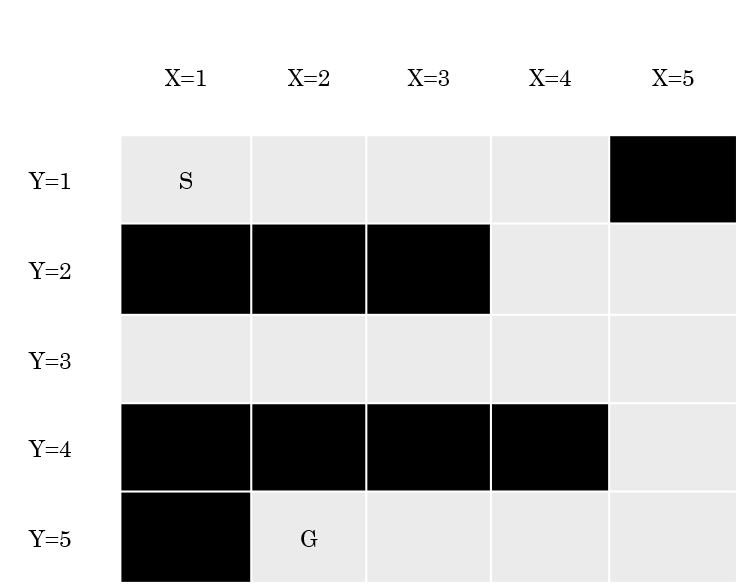
\includegraphics[scale=0.7]{img/ourMaze.png}
    \caption{The analyzed Maze}\label{fig:our}
\end{figure}

\begin{lstlisting}[label={lst:r_tr}, language=Prolog, caption=\texttt{reach/3} with tail recursion, belowcaptionskip=1cm]
reach(A,B,L) :- reach_1(A,B,[A],L).
reach_1(A,A,L,L).
reach_1(A,B,Acc,L) :-
    move(A,C),
    non_member(C,Acc),
    reach_1(C,B,[C|Acc],L). 
\end{lstlisting}
This procedure resembles the techniques for a loop preventing Depth-First Search. The idea behind this procedure is to store
the already visited cells into an accumulator (\texttt{Acc}), and, at each step, check whether a new encountered cell has already
been visited before.\\
Unfortunately, we were not able to learn this procedure through any of the mentioned ILP techniques.
